\documentclass[11pt]{article}
\usepackage[utf8]{inputenc}
\usepackage[T1]{fontenc}
\usepackage[margin=1in]{geometry}
\usepackage{amsmath,amssymb,amsthm}
\usepackage{graphicx}
\usepackage{booktabs}
\usepackage{hyperref}
\usepackage{listings}
\usepackage{xcolor}
\hypersetup{colorlinks=true, linkcolor=blue, citecolor=blue, urlcolor=blue}

\lstdefinelanguage{Lean4}{
  morekeywords={theorem,def,noncomputable,import,namespace,end,open,by,fun},
  morecomment=[l]{--},
  morecomment=[s]{/-}{-/},
  sensitive=true,
}
\lstset{basicstyle=\small\ttfamily, language=Lean4, columns=fullflexible, breaklines=true}

% Every number from this run is a macro generated from results/bao_bbn_h0/*.json
% (and the published targets from results/bao_bbn_h0/preregistration.json) by
% scripts/bao_bbn_h0/make_paper_inputs.py. Nothing numeric from the fit is typed here.
% generated by scripts/bao_bbn_h0/make_paper_inputs.py -- do not edit
\newcommand{\AgFlags}{74}
\newcommand{\AgOwnCamb}{0}
\newcommand{\AgOwnFlags}{0}
\newcommand{\AgStatus}{FAIL}
\newcommand{\AmendTime}{2026-09-27 16:04:27}
\newcommand{\AnchorCambTwo}{147.1027}
\newcommand{\AnchorClassMatched}{147.1071}
\newcommand{\AnchorClassMatchedNeff}{3.044}
\newcommand{\AnchorClassNeff}{3.046}
\newcommand{\AnchorClassTwo}{147.0971}
\newcommand{\AnchorMatchedFrac}{\ensuremath{3.0\times10^{-5}}}
\newcommand{\AubMax}{\ensuremath{+0.006}}
\newcommand{\AubMaxAbs}{0.029}
\newcommand{\AubMin}{\ensuremath{-0.029}}
\newcommand{\BbnMean}{0.02218}
\newcommand{\BbnSig}{0.00055}
\newcommand{\BgMax}{\ensuremath{1.2\times10^{-6}}}
\newcommand{\CambAnchor}{147.0492}
\newcommand{\CambOrch}{147.1027}
\newcommand{\CambVer}{2.0.4}
\newcommand{\ClassMax}{\ensuremath{7.0\times10^{-5}}}
\newcommand{\ClassOrch}{147.0971}
\newcommand{\DPrimSecOne}{\ensuremath{-0.034}}
\newcommand{\DPrimSecTwo}{\ensuremath{-0.004}}
\newcommand{\FitShaShort}{8974d5d29ad7bb5b}
\newcommand{\GOneChi}{10.28}
\newcommand{\GOneCorr}{\ensuremath{-0.93}}
\newcommand{\GOneDof}{11}
\newcommand{\GOneHrd}{101.52}
\newcommand{\GOneHrdErr}{0.74}
\newcommand{\GOneOm}{0.2977}
\newcommand{\GOneOmErr}{0.0087}
\newcommand{\GOnePassed}{passed}
\newcommand{\GOnePte}{0.51}
\newcommand{\GOnePullHrd}{\ensuremath{-0.027}}
\newcommand{\GOnePullOm}{0.024}
\newcommand{\GRadH}{0.6851}
\newcommand{\GTwoChi}{12.74}
\newcommand{\GTwoCorr}{\ensuremath{-0.92}}
\newcommand{\GTwoDof}{10}
\newcommand{\GTwoHrd}{101.93}
\newcommand{\GTwoHrdErr}{1.27}
\newcommand{\GTwoOm}{0.2945}
\newcommand{\GTwoOmErr}{0.0145}
\newcommand{\GTwoPassed}{passed}
\newcommand{\GTwoPte}{0.24}
\newcommand{\GTwoPullHrd}{0.103}
\newcommand{\GTwoPullOm}{\ensuremath{-0.033}}
\newcommand{\HDep}{\ensuremath{2.1\times10^{-4}}}
\newcommand{\HDepArgH}{0.2}
\newcommand{\HDepCore}{\ensuremath{1.8\times10^{-5}}}
\newcommand{\InterpCoreMax}{\ensuremath{3.1\times10^{-5}}}
\newcommand{\InterpCoreN}{200}
\newcommand{\InterpCoreRms}{\ensuremath{2.3\times10^{-6}}}
\newcommand{\InterpWideMax}{\ensuremath{6.4\times10^{-6}}}
\newcommand{\InterpWideN}{100}
\newcommand{\LeanNThm}{10}
\newcommand{\LeanShaShort}{2b6530838efa0df9}
\newcommand{\LedgerBlock}{0}
\newcommand{\LedgerClaims}{43}
\newcommand{\LedgerFlag}{2}
\newcommand{\LedgerRc}{1}
\newcommand{\LockedDiffOne}{0.0}
\newcommand{\LockedDiffTwo}{0.0}
\newcommand{\LockedHOne}{68.579}
\newcommand{\LockedHOneErr}{0.601}
\newcommand{\LockedHTwo}{68.701}
\newcommand{\LockedHTwoErr}{0.815}
\newcommand{\LockedOmOne}{0.2976}
\newcommand{\LockedSha}{b7fe5608e4ae6d0b}
\newcommand{\MonoAllOk}{all}
\newcommand{\MonoBelowDec}{strictly decreasing}
\newcommand{\MonoN}{300}
\newcommand{\MonoThr}{0.0013}
\newcommand{\NFourCaught}{exceeds}
\newcommand{\NFourDchi}{\ensuremath{5.2\times10^{-5}}}
\newcommand{\NFourShift}{\ensuremath{+0.164}}
\newcommand{\NGrid}{8967}
\newcommand{\NOneChiP}{\ensuremath{1.43\times10^{5}}}
\newcommand{\NOneChiS}{\ensuremath{1.35\times10^{5}}}
\newcommand{\NOnePte}{0.0}
\newcommand{\NOneRealPte}{0.505}
\newcommand{\NSubst}{22}
\newcommand{\NThreeRatioP}{20.99}
\newcommand{\NThreeRatioS}{21.71}
\newcommand{\NThreeSigP}{12.5}
\newcommand{\NThreeSigS}{13.1}
\newcommand{\NThreeStepsP}{40000}
\newcommand{\NThreeStepsS}{88000}
\newcommand{\NThreeStepsTauP}{582}
\newcommand{\NThreeStepsTauS}{68}
\newcommand{\NThreeTauP}{69}
\newcommand{\NThreeTauS}{1300}
\newcommand{\NTwoChiP}{1420.2}
\newcommand{\NTwoChiS}{1420.2}
\newcommand{\NTwoDof}{12}
\newcommand{\NTwoPte}{\ensuremath{6.2\times10^{-297}}}
\newcommand{\NeffOffsetPct}{0.0065}
\newcommand{\PFour}{\ensuremath{1.7\times10^{-6}}}
\newcommand{\POneHp}{\ensuremath{+0.0041}}
\newcommand{\POneHs}{\ensuremath{+0.0035}}
\newcommand{\POneOmp}{\ensuremath{+0.0006}}
\newcommand{\POneOms}{\ensuremath{+0.0005}}
\newcommand{\PTOneChi}{10.28}
\newcommand{\PTOneCorr}{0.74}
\newcommand{\PTOneDH}{0.035}
\newcommand{\PTOneDof}{11}
\newcommand{\PTOneEss}{3109}
\newcommand{\PTOneH}{68.55}
\newcommand{\PTOneHErr}{0.59}
\newcommand{\PTOneHErrthree}{0.594}
\newcommand{\PTOneHrd}{101.52}
\newcommand{\PTOneHrdErr}{0.73}
\newcommand{\PTOneHthree}{68.545}
\newcommand{\PTOneLapH}{0.60}
\newcommand{\PTOneMapH}{68.53}
\newcommand{\PTOneOm}{0.2977}
\newcommand{\PTOneOmErr}{0.0085}
\newcommand{\PTOneProfHi}{69.13}
\newcommand{\PTOneProfLo}{67.93}
\newcommand{\PTOneProfSig}{0.60}
\newcommand{\PTOnePte}{0.51}
\newcommand{\PTOnePullH}{0.06}
\newcommand{\PTOnePullOm}{\ensuremath{-0.0005}}
\newcommand{\PTOneRd}{148.1}
\newcommand{\PTOneRdErr}{1.6}
\newcommand{\PTOneSigRatio}{1.024}
\newcommand{\PTOneSteps}{4000}
\newcommand{\PTOneTau}{39}
\newcommand{\PTOneVerdict}{PASS}
\newcommand{\PTOneWb}{0.02219}
\newcommand{\PTOneWbErr}{0.00055}
\newcommand{\PTTwoChi}{12.74}
\newcommand{\PTTwoCorr}{0.55}
\newcommand{\PTTwoDH}{0.167}
\newcommand{\PTTwoDof}{10}
\newcommand{\PTTwoEss}{3353}
\newcommand{\PTTwoH}{68.70}
\newcommand{\PTTwoHErr}{0.81}
\newcommand{\PTTwoHErrthree}{0.809}
\newcommand{\PTTwoHrd}{101.84}
\newcommand{\PTTwoHrdErr}{1.26}
\newcommand{\PTTwoHthree}{68.697}
\newcommand{\PTTwoLapH}{0.81}
\newcommand{\PTTwoMapH}{68.64}
\newcommand{\PTTwoOm}{0.2953}
\newcommand{\PTTwoOmErr}{0.0146}
\newcommand{\PTTwoProfHi}{69.46}
\newcommand{\PTTwoProfLo}{67.84}
\newcommand{\PTTwoProfSig}{0.81}
\newcommand{\PTTwoPte}{0.24}
\newcommand{\PTTwoPullH}{0.21}
\newcommand{\PTTwoPullOm}{0.0215}
\newcommand{\PTTwoRd}{148.3}
\newcommand{\PTTwoRdErr}{2.4}
\newcommand{\PTTwoSigRatio}{1.012}
\newcommand{\PTTwoSteps}{4000}
\newcommand{\PTTwoTau}{36}
\newcommand{\PTTwoVerdict}{PARTIAL}
\newcommand{\PTTwoWb}{0.02220}
\newcommand{\PTTwoWbErr}{0.00055}
\newcommand{\PTwoChiP}{10.95}
\newcommand{\PTwoMeanP}{\ensuremath{-0.064}}
\newcommand{\PTwoMeanS}{\ensuremath{-0.067}}
\newcommand{\PTwoN}{100}
\newcommand{\PTwoOmMeanP}{\ensuremath{-0.131}}
\newcommand{\PTwoOmStdP}{0.944}
\newcommand{\PTwoStdP}{1.023}
\newcommand{\PTwoStdS}{1.025}
\newcommand{\PreregShaShort}{5bcde156f38c2218}
\newcommand{\PreregTime}{2026-09-27 15:53:42}
\newcommand{\PropEight}{0.18}
\newcommand{\PropNine}{0.05}
\newcommand{\PropSlopeTwo}{0.492}
\newcommand{\PyResult}{collection was interrupted by 21 errors, all \texttt{ModuleNotFoundError} for \texttt{fastapi}, \texttt{peft}, \texttt{radon}, \texttt{starlette} (the worktree venv lacks the optional extras), so no test ran}
\newcommand{\RebInterp}{0.004}
\newcommand{\RebMc}{0.05}
\newcommand{\RebStrict}{0.050}
\newcommand{\RebTOne}{passes}
\newcommand{\RebTTwo}{fails}
\newcommand{\RigorFiles}{141}
\newcommand{\Runtime}{388}
\newcommand{\STOneChi}{10.28}
\newcommand{\STOneCorr}{0.74}
\newcommand{\STOneDH}{0.069}
\newcommand{\STOneDof}{11}
\newcommand{\STOneEss}{3139}
\newcommand{\STOneH}{68.58}
\newcommand{\STOneHErr}{0.60}
\newcommand{\STOneHErrthree}{0.601}
\newcommand{\STOneHrd}{101.54}
\newcommand{\STOneHrdErr}{0.73}
\newcommand{\STOneHthree}{68.579}
\newcommand{\STOneLapH}{0.60}
\newcommand{\STOneMapH}{68.57}
\newcommand{\STOneOm}{0.2976}
\newcommand{\STOneOmErr}{0.0086}
\newcommand{\STOneProfHi}{69.16}
\newcommand{\STOneProfLo}{67.97}
\newcommand{\STOneProfSig}{0.60}
\newcommand{\STOnePte}{0.51}
\newcommand{\STOnePullH}{0.12}
\newcommand{\STOnePullOm}{\ensuremath{-0.0151}}
\newcommand{\STOneRd}{148.1}
\newcommand{\STOneRdErr}{1.6}
\newcommand{\STOneSigRatio}{1.037}
\newcommand{\STOneSteps}{4000}
\newcommand{\STOneTau}{39}
\newcommand{\STOneVerdict}{PASS}
\newcommand{\STOneWb}{0.02218}
\newcommand{\STOneWbErr}{0.00055}
\newcommand{\STTwoChi}{12.74}
\newcommand{\STTwoCorr}{0.55}
\newcommand{\STTwoDH}{0.171}
\newcommand{\STTwoDof}{10}
\newcommand{\STTwoEss}{3239}
\newcommand{\STTwoH}{68.70}
\newcommand{\STTwoHErr}{0.81}
\newcommand{\STTwoHErrthree}{0.815}
\newcommand{\STTwoHrd}{101.91}
\newcommand{\STTwoHrdErr}{1.25}
\newcommand{\STTwoHthree}{68.701}
\newcommand{\STTwoLapH}{0.81}
\newcommand{\STTwoMapH}{68.68}
\newcommand{\STTwoOm}{0.2946}
\newcommand{\STTwoOmErr}{0.0143}
\newcommand{\STTwoProfHi}{69.50}
\newcommand{\STTwoProfLo}{67.87}
\newcommand{\STTwoProfSig}{0.81}
\newcommand{\STTwoPte}{0.24}
\newcommand{\STTwoPullH}{0.21}
\newcommand{\STTwoPullOm}{\ensuremath{-0.0282}}
\newcommand{\STTwoRd}{148.4}
\newcommand{\STTwoRdErr}{2.3}
\newcommand{\STTwoSigRatio}{1.018}
\newcommand{\STTwoSteps}{4000}
\newcommand{\STTwoTau}{38}
\newcommand{\STTwoVerdict}{PARTIAL}
\newcommand{\STTwoWb}{0.02218}
\newcommand{\STTwoWbErr}{0.00055}
\newcommand{\SensEqTwo}{\ensuremath{+0.049}}
\newcommand{\SensNeff}{\ensuremath{+4.65}}
\newcommand{\SensNoRadP}{\ensuremath{+0.031}}
\newcommand{\SensNoRadS}{\ensuremath{-0.003}}
\newcommand{\SlopeP}{0.491}
\newcommand{\SysStrict}{0.139}
\newcommand{\TTwoMarginP}{0.017}
\newcommand{\TTwoMarginS}{0.021}
\newcommand{\TTwoMcP}{0.014}
\newcommand{\TTwoMcS}{0.014}
\newcommand{\TTwoResRatioP}{1.1}
\newcommand{\TTwoResRatioS}{1.4}
\newcommand{\TgGOneCorr}{\ensuremath{-0.92}}
\newcommand{\TgGOneHrd}{101.54}
\newcommand{\TgGOneHrdErr}{0.73}
\newcommand{\TgGOneOm}{0.2975}
\newcommand{\TgGOneOmErr}{0.0086}
\newcommand{\TgGTwoHrd}{101.8}
\newcommand{\TgGTwoHrdErr}{1.3}
\newcommand{\TgGTwoOm}{0.295}
\newcommand{\TgGTwoOmErr}{0.015}
\newcommand{\TgTOneH}{68.51}
\newcommand{\TgTOneHErr}{0.58}
\newcommand{\TgTOneOm}{0.2977}
\newcommand{\TgTOneOmErr}{0.0086}
\newcommand{\TgTTwoH}{68.53}
\newcommand{\TgTTwoHErr}{0.80}
\newcommand{\TgTTwoOm}{0.295}
\newcommand{\TgTTwoOmErr}{0.015}
\newcommand{\TolSoft}{0.33}
\newcommand{\TolStrict}{0.15}
\newcommand{\TolStrictSig}{0.26}


\title{An Inverse Distance Ladder from Public DESI BAO:\\
$H_0$ from DESI DR2 BAO plus a BBN $\omega_b$ Prior,\\
with an Exact Boltzmann-Code Sound Horizon}
\author{AutoevolveAI / ANSE Research Pipeline \\
\small Generated with Claude Code; model-produced. The model name recorded by \\
\small the generating session (Claude Opus 5.5) is an unverifiable statement: \\
\small no artifact can confirm which model produced earlier stages. \\
\small Not reviewed by a person}
\date{September 27, 2026}

\begin{document}
\sloppy
\maketitle

\begin{abstract}
We reproduce the DESI inverse-distance-ladder measurement of the Hubble
constant. The inputs are the public DESI DR2 Gaussian BAO summary
statistics \cite{desi2025dr2} and a Big-Bang-nucleosynthesis prior
$\omega_b=\BbnMean\pm\BbnSig$. No CMB anisotropy or $\theta_*$
information enters. The fit assumes
flat $\Lambda$CDM with standard pre-recombination physics.

The analysis was preregistered with a fitting-formula sound horizon. A
protocol amendment then made an exact CAMB~\CambVer{} $r_d$ the primary
analysis, cross-checked with CLASS. The preregistered fitting formula is
kept as the secondary analysis.

The primary analysis gives
$H_0=\PTOneH\pm\PTOneHErr$~km\,s$^{-1}$\,Mpc$^{-1}$ and
$\Omega_m=\PTOneOm\pm\PTOneOmErr$. The published values are
$\TgTOneH\pm\TgTOneHErr$ and $\TgTOneOm\pm\TgTOneOmErr$. The preregistered
verdict is \textbf{\PTOneVerdict}: $|\Delta H_0|=\PTOneDH$, against a strict
tolerance of \TolStrict{}.

The DESI DR1 second check is \textbf{\PTTwoVerdict}. It gives
$H_0=\PTTwoH\pm\PTTwoHErr$ against the published $\TgTTwoH\pm\TgTTwoHErr$.
$|\Delta H_0|=\PTTwoDH$ exceeds the strict \TolStrict{} but lies within the
soft \TolSoft{}~km\,s$^{-1}$\,Mpc$^{-1}$. It crosses the strict limit by
\TTwoMarginP, which is about \TTwoResRatioP{} times our Monte-Carlo error on
the mean combined with the rounding of the published value, so the
PASS/PARTIAL boundary is not statistically resolved.

The secondary analysis gives the same verdicts: T1 \STOneVerdict{} with
$H_0=\STOneH\pm\STOneHErr$, and T2 \STTwoVerdict. It is bit-identical to a
hash-locked fit that was written before the amendment.

Four positive controls and three negative controls behave as preregistered
(P2 with one clarification declared before it ran). N1 and N2 would fail
for almost any pipeline; a post-hoc control added after review (N4, a
neutrino-bookkeeping error in $r_d$) shifts $H_0$ by \NFourShift{} and is
invisible to the data ($|\Delta\chi^2|=\NFourDchi$).
The BAO-only gate reproduces DESI's $(\Omega_m, h r_d)$ with pulls
$\GOnePullOm\sigma$ and $\GOnePullHrd\sigma$. \LeanNThm{} Lean~4 theorems about
the model as coded are kernel-checked with only the trusted axioms. Six
are substantive: positivity of the eq.~16 sound horizon, three
strict-monotonicity results on the sampled support, and the preregistered
identifiability statement that $h\,r_d(h)$ is strictly increasing in $h$
(with its generic lemma). The other four are the positivity of a constant
and three field identities.

This is a reproduction of a published number from its own public inputs.
It is not a new constraint.
\end{abstract}

\section{Introduction}

BAO measure $D_M(z)/r_d$, $D_H(z)/r_d=c/[H(z)r_d]$ and
$D_V(z)/r_d$. In flat $\Lambda$CDM these fix $\Omega_m$ and the product
$h r_d$, but not $h$ and $r_d$ separately. With standard early-universe
physics, $r_d$ is a function of $(\omega_b,\omega_{cb})$. A BBN prior on
$\omega_b$ therefore calibrates the ruler and yields $H_0$ without the CMB
acoustic scale \cite{desi2025dr2,schoeneberg2022}. DESI DR2 reports
$H_0=\TgTOneH\pm\TgTOneHErr$ (eq.~19 and Table~V) and DESI DR1 reports
$\TgTTwoH\pm\TgTTwoHErr$ \cite{desi2024vi}. We re-derive both from the
released summary statistics and treat agreement as an external correctness
test of the pipeline. We then state what the agreement does and does not show.

\section{Data}

We use \texttt{desi\_gaussian\_bao\_ALL\_GCcomb\_\{mean,cov\}.txt} from
DESI DR2: 13 points and a full $13\times13$ covariance
(Table~\ref{tab:dr2}). For DR1 we use
\texttt{desi\_2024\_gaussian\_bao\_ALL\_GCcomb\_\{mean,cov\}.txt}: 12
points, DESI only, no SDSS \cite{desi2024vi}. The sha256 of all four files
was fixed in the preregistration before any fit and re-verified by the fit
script. They are recorded in \texttt{results/bao\_bbn\_h0/fit.json}.

\begin{table}[h]
\centering
\caption{DESI DR2 BAO data (values and $\sqrt{\mathrm{diag}\,C}$ read from the data files).}
\label{tab:dr2}
\begin{tabular}{cccc}
\toprule
$z_\mathrm{eff}$ & Quantity & Value & $\sigma$ \\
\midrule
0.295 & $D_V/r_d$ & 7.942 & 0.076 \\
0.510 & $D_M/r_d$ & 13.588 & 0.168 \\
0.510 & $D_H/r_d$ & 21.863 & 0.429 \\
0.706 & $D_M/r_d$ & 17.351 & 0.180 \\
0.706 & $D_H/r_d$ & 19.455 & 0.334 \\
0.934 & $D_M/r_d$ & 21.576 & 0.162 \\
0.934 & $D_H/r_d$ & 17.641 & 0.201 \\
1.321 & $D_M/r_d$ & 27.601 & 0.325 \\
1.321 & $D_H/r_d$ & 14.176 & 0.225 \\
1.484 & $D_M/r_d$ & 30.512 & 0.764 \\
1.484 & $D_H/r_d$ & 12.817 & 0.518 \\
2.330 & $D_H/r_d$ & 8.632 & 0.101 \\
2.330 & $D_M/r_d$ & 38.989 & 0.532 \\
\bottomrule
\end{tabular}

\end{table}

\begin{table}[h]
\centering
\caption{DESI DR1 BAO data used for the second check (read from the data files).}
\label{tab:dr1}
\begin{tabular}{cccc}
\toprule
$z_\mathrm{eff}$ & Quantity & Value & $\sigma$ \\
\midrule
0.295 & $D_V/r_d$ & 7.925 & 0.151 \\
0.510 & $D_M/r_d$ & 13.620 & 0.252 \\
0.510 & $D_H/r_d$ & 20.983 & 0.611 \\
0.706 & $D_M/r_d$ & 16.846 & 0.319 \\
0.706 & $D_H/r_d$ & 20.079 & 0.595 \\
0.930 & $D_M/r_d$ & 21.708 & 0.282 \\
0.930 & $D_H/r_d$ & 17.876 & 0.346 \\
1.317 & $D_M/r_d$ & 27.787 & 0.690 \\
1.317 & $D_H/r_d$ & 13.824 & 0.422 \\
1.491 & $D_V/r_d$ & 26.072 & 0.669 \\
2.330 & $D_M/r_d$ & 39.708 & 0.943 \\
2.330 & $D_H/r_d$ & 8.523 & 0.171 \\
\bottomrule
\end{tabular}

\end{table}

\section{Model and method}

\paragraph{Parameters and priors.}
We sample $(H_0,\omega_b,\Omega_m)$ with emcee (32 walkers). The flat
priors are $H_0\in[20,100]$, $\omega_b\in[0.005,0.1]$ and
$\Omega_m\in[0.01,0.99]$, as in DESI DR1 Table~2 \cite{desi2024vi}, which
DR2 adopts \cite{desi2025dr2}. On top of these sits the Gaussian BBN prior
$\omega_b=\BbnMean\pm\BbnSig$ \cite{desi2025dr2,schoeneberg2024}. We fix
$N_\mathrm{eff}=3.044$, one massive neutrino of 0.06~eV, and
$T_\mathrm{CMB}=2.7255$~K. $\Omega_m$ includes the massive neutrino.

We run until $N_\mathrm{steps}>50\tau$ for every parameter and discard
$5\tau$ as burn-in. The reported statistic is the posterior mean and
standard deviation, as in DR2 Table~V. We also report the MAP, a Laplace
width and a profile likelihood.

\paragraph{Background.}
$D_M$ and $D_H$ come from a Gauss--Legendre integrator of
$E(z)=[\Omega_m(1+z)^3+\Omega_r(1+z)^4+1-\Omega_m-\Omega_r]^{1/2}$. Here
$\Omega_r$ holds the photons and the massless share of $N_\mathrm{eff}$,
and the 0.06~eV neutrino is counted as matter. This background agrees with
astropy \texttt{FlatLambdaCDM} to \PFour{} (control P4). It agrees with
CAMB's own background $D_M$ and $D_H$ to \BgMax{}.

\paragraph{Primary sound horizon (amendment 1).}
$r_\mathrm{drag}$ is computed with CAMB~\CambVer{} at $N_\mathrm{eff}=3.044$
with one massive neutrino, on a $49\times61\times3$ grid in
$(\ln\omega_b,\ln\omega_{cdm},h)$ (\NGrid{} nodes). The interpolant is a
bicubic spline in $\ln r_\mathrm{drag}$ at each $h$ node, linear in $h$.
It matches direct CAMB calls to a maximum of \InterpCoreMax{} (rms
\InterpCoreRms{}) at \InterpCoreN{} core points, and to \InterpWideMax{}
at \InterpWideN{} wide-range points. CLASS~3.3.4 agrees with CAMB to at
most \ClassMax{} at five points, which include the BBN $\pm2\sigma$ edges.

\NSubst{} nodes failed in CAMB's recombination solver. All of them sit at
the $h=0.99$ node with very low $\Omega_m$. They were refilled with CAMB at
$h=0.98$, and every refilled node is listed in
\texttt{rd\_camb\_validation.json}.

At fixed physical densities, the table's $r_\mathrm{drag}$ varies across
its $h$ nodes by at most \HDepCore{} in the core region. The largest
variation, \HDep, is at the $h=\HDepArgH$ node in a far corner of the grid,
not at a refilled node.

At the Planck 2018 Table~1 best-fit inputs ($N_\mathrm{eff}=3.046$) the
instrument gives $r_\mathrm{drag}=\CambAnchor$~Mpc. That reproduces the
published 147.049~Mpc \cite{planck2018}.

\paragraph{Secondary sound horizon (preregistered).}
The secondary analysis uses Aubourg et al.\ eq.~16 \cite{aubourg2015}:
\begin{equation}
r_d \simeq \frac{55.154\,e^{-72.3(\omega_\nu+0.0006)^2}}{\omega_{cb}^{0.25351}\,\omega_b^{0.12807}}~\mathrm{Mpc},\qquad
\omega_\nu=0.0107\times0.06,\quad \omega_{cb}=\Omega_m h^2-\omega_\nu .
\label{eq:aub}
\end{equation}
Its stated accuracy is 0.021\% for $N_\mathrm{eff}=3.046$ within
$3\sigma$ of Planck \cite{aubourg2015}. We measured eq.~\eqref{eq:aub}
against CAMB at $N_\mathrm{eff}=3.044$ at the five cross-check points. The
difference ranges from \AubMin\% to \AubMax\%. Its magnitude reaches
\AubMaxAbs\%, which is above the stated 0.021\%. About \NeffOffsetPct\% of that is
the uncorrected $N_\mathrm{eff}$ offset from Aubourg's eq.~17. The rest is
unexplained here.

\paragraph{BAO-only gate.}
Gates G1 (DR2) and G2 (DR1) sample $(\Omega_m, h r_d)$ with no $r_d$ model
and $h r_d\in[10,1000]$. The radiation term is evaluated at a fixed
$h=\GRadH$. These gates are the external positive control against DESI's
own pipeline.

\section{Preregistration, amendment and locked output}

The preregistration (\texttt{preregistration.json}, sha256
\texttt{\PreregShaShort\ldots}, \PreregTime{} UTC) fixed these choices
before any fit: targets, priors, statistic, $r_d$ method, controls and
tolerances.

\paragraph{Tolerances.}
DESI used the same data vector, BBN prior and flat priors. The published
$\sigma$ is therefore not independent noise on the difference, so the
tolerances were built from a systematic budget instead:
\begin{itemize}
\item \textbf{Strict:} \TolStrict{}~km\,s$^{-1}$\,Mpc$^{-1}$. This is a
  0.10\% $r_d$-formula proxy (\SysStrict) added in quadrature to a 0.05
  Monte-Carlo allowance, i.e.\ $\TolStrictSig\sigma$ of T1.
\item \textbf{Soft:} \TolSoft{}~km\,s$^{-1}$\,Mpc$^{-1}$, from the maximum
  0.233\% difference between two $r_d$ formulas over the prior box.
\end{itemize}
Amendment~1 kept these tolerances unchanged, but the 0.139 formula term
no longer applies to the primary analysis, which uses CAMB. With only the
preregistered Monte-Carlo allowance (\RebMc) and the measured table
interpolation error propagated to $H_0$ (\RebInterp), the strict budget
for the primary would be \RebStrict~km\,s$^{-1}$\,Mpc$^{-1}$. The
preregistered strict limit of \TolStrict{} is therefore generous for the
primary. We apply the preregistered rule unchanged. For information, under
the re-derived \RebStrict{} T1 \RebTOne{} and T2 \RebTTwo{}
(Sec.~\ref{sec:t2}).

\paragraph{Verdict rule.}
PASS requires all of the following:
\begin{itemize}
\item $|H_0-\TgTOneH|\le\TolStrict$;
\item $|\Omega_m-\TgTOneOm|\le0.25\times\TgTOneOmErr$;
\item $\sigma(H_0)$ within $\pm15\%$ of \TgTOneHErr;
\item gate G1 passes;
\item every control behaves.
\end{itemize}
PARTIAL means $\TolStrict<|\Delta H_0|\le\TolSoft$ with the other
conditions met. The headline verdict is T1. T2 (DR1) is reported
separately under the same thresholds.

\paragraph{Timeline of the amendment.}
The events, taken from the amendment file:
\begin{itemize}
\item CAMB, CLASS and cobaya were installed after the preregistration was
  written.
\item A fitting-formula fit output was written at 16:03:03~UTC.
\item Amendment~1 was filed at \AmendTime{} UTC. It made the exact CAMB
  $r_d$ primary and kept the fitting formula as the secondary analysis.
  Targets, tolerances and controls were unchanged.
\item The amender states that the earlier output was not read. This is an
  assertion that no hash can prove; we label it unverifiable. Both
  analyses give the same verdicts, so no selection between them was
  possible. The output was
  hash-locked and renamed
  (\texttt{fit\_attempt1\_fittingformula\_UNREAD\_AT\_AMENDMENT.json},
  sha256 \texttt{\LockedSha\ldots}).
\end{itemize}

\paragraph{The locked output.}
It contains T1 $H_0=\LockedHOne\pm\LockedHOneErr$ and T2
$H_0=\LockedHTwo\pm\LockedHTwoErr$. Our re-run secondary analysis
reproduces it bit for bit: the differences are \LockedDiffOne{} (T1) and
\LockedDiffTwo{} (T2), and G1 and G2 are identical. The seeds and code path
are fixed, so this shows reproducibility, not independent correctness.

The amendment's reason quotes a CAMB positive control of \CambOrch~Mpc, a
CLASS value of \ClassOrch~Mpc, and a published Planck 2018 value of
$147.09\pm0.26$. That published value is the posterior mean in
\cite{planck2018} Table~1 (column ``Plik [1]'', the same row as the
147.049 best fit) and Table~2 (TT,TE,EE+lowE+lensing); \cite{desi2024vi}
quotes it before its eq.~(4.3). Both code values are reproduced at the
Table~2 TT,TE,EE+lowE+lensing means ($H_0=67.36$, $\omega_b=0.02237$,
$\omega_c=0.1200$, one 0.06~eV neutrino). CAMB with $N_\mathrm{eff}=3.044$
gives \AnchorCambTwo~Mpc. CLASS with \texttt{N\_ur}$\,=2.0328$ gives
\AnchorClassTwo~Mpc, but CLASS reports $N_\mathrm{eff}=\AnchorClassNeff$
for that setting. So the amendment's two numbers are not at the same
$N_\mathrm{eff}$. At matched $N_\mathrm{eff}=\AnchorClassMatchedNeff$
(\texttt{N\_ur}$\,=2.0308$, the setting used for our CLASS cross-check)
CLASS gives \AnchorClassMatched~Mpc, a fractional difference of
\AnchorMatchedFrac{} from CAMB. The ledger stage re-ran these CAMB and
CLASS evaluations; they are bit-identical to the rows recorded in
\texttt{fit.json}. An earlier draft of this paper said the anchor could not
be reproduced and that 147.09 was not in the fetched sources. Both
statements were wrong and were corrected.

\section{Controls}

Each control was run for both analyses before the target comparison.

\begin{itemize}
\item \textbf{P1, noiseless mock} (truth $H_0=68$, $\Omega_m=0.300$,
  $\omega_b=0.02218$; rule $|\Delta H_0|\le0.1$, $|\Delta\Omega_m|\le0.002$).
  Primary: $\Delta H_0=\POneHp$, $\Delta\Omega_m=\POneOmp$.
  Secondary: $\Delta H_0=\POneHs$, $\Delta\Omega_m=\POneOms$.
  Passed.
\item \textbf{P2, \PTwoN{} noisy mocks, MAP per mock} (rule: mean $H_0$
  pull within $\pm0.2$, width in $[0.8,1.2]$). Primary: mean
  $\PTwoMeanP$, width $\PTwoStdP$. Secondary: mean $\PTwoMeanS$, width
  $\PTwoStdS$. The primary $\Omega_m$ pull is $\PTwoOmMeanP$/$\PTwoOmStdP$
  and the mean $\chi^2$ is \PTwoChiP{} for 11 dof. Passed.
  \emph{Deviation, written before P2 first ran:} each mock also draws the
  BBN centre from $\mathcal{N}(\BbnMean,\BbnSig)$. Without that draw the
  pull width is below~1 by construction.
\item \textbf{P3 = gate G1}: \GOnePassed{} (Table~\ref{tab:res}).
  G2 also \GTwoPassed.
\item \textbf{P4, predictor cross-check}: astropy against the manual
  integrator, maximum fractional difference \PFour{} (threshold $10^{-4}$).
  Passed.
\item \textbf{N1, scrambled DR2 vector} (fixed seed): $\chi^2=\NOneChiP$
  (primary) and \NOneChiS{} (secondary), PTE \NOnePte. The real data give
  PTE \NOneRealPte. Behaves.
\item \textbf{N2, Einstein--de Sitter} on the real data:
  $\chi^2=\NTwoChiP$ for \NTwoDof{} dof, PTE \NTwoPte. Behaves.
\item \textbf{N3, no BBN prior} (rule: $\sigma(H_0)$ grows more than
  $5\times$): $\sigma(H_0)$ grows $\NThreeRatioP\times$ (primary) and
  $\NThreeRatioS\times$ (secondary). Behaves.
  \begin{itemize}
  \item The primary chain ran \NThreeStepsP{} steps with
    $\tau_\mathrm{max}\approx\NThreeTauP$ ($N/\tau\approx\NThreeStepsTauP$).
  \item The secondary chain ran \NThreeStepsS{} steps with
    $\tau_\mathrm{max}\approx\NThreeTauS$ ($N/\tau\approx\NThreeStepsTauS$).
    A $\tau$ estimate for such a broad, prior-truncated posterior is not
    reliable, so the 50-$\tau$ criterion is nominal here. The control's
    conclusion does not depend on it: the ratio is far above 5.
  \item The posterior fills the flat priors. The CAMB table's support
    ($h\le0.99$, $\omega_{cdm}\ge0.005$) truncates the primary prior, and
    this matters only for N3.
  \end{itemize}
\end{itemize}

The preregistration's report rules mention N1--N4, but only N1--N3 are
defined. The $N_\mathrm{eff}=4.044$ run is a sensitivity demonstration, not
a control.

\paragraph{What the controls do and do not show.}
P1 and P2 use the same predictor that generated the mocks, so they test
self-consistency, not correctness. N1 ($\chi^2\sim10^5$) and N2 would fail
for almost any pipeline, including one with a wrong $r_d$ convention or a
wrong neutrino treatment. Of the preregistered controls, only N3 is
informative, and its ratio depends on the prior box, which the CAMB table
truncates for the primary. The external checks are G1/G2, the T1/T2
comparisons themselves, and the CLASS-versus-CAMB $r_d$ cross-check.
``All controls behave'' should not be read as more than that.

\paragraph{N4, post-hoc wrong-convention control (not preregistered).}
N4 was added after review. It is not part of the verdict's controls
condition. Its expectation and pass rule were written to
\texttt{controls/N4\_expectation.json} before it ran. N4 evaluates the
primary CAMB $r_d$ with $\omega_{cdm}=\Omega_m h^2-\omega_b$, forgetting to
subtract the massive-neutrino density. On the DR2 BAO+BBN likelihood it
shifts the MAP $H_0$ by \NFourShift~km\,s$^{-1}$\,Mpc$^{-1}$, which
\NFourCaught{} the strict \TolStrict. The fit quality is unchanged
($|\Delta\chi^2|=\NFourDchi$). So the data cannot detect this error; only
the external comparison can, and only by a narrow margin over the strict
limit. The soft tolerance would not catch it.

\section{Results}

\begin{table}[h]
\centering
\caption{Posterior means $\pm$ standard deviations (emcee), against the published values.
$|\Delta H_0|$ is in km\,s$^{-1}$\,Mpc$^{-1}$. All entries are generated from \texttt{fit.json}.}
\label{tab:res}
\small\setlength{\tabcolsep}{4pt}
\begin{tabular}{llcccc}
\toprule
Target & Analysis & $H_0$ & $\Omega_m$ & $|\Delta H_0|$ & Verdict \\
\midrule
T1 DR2+BBN & primary (CAMB)   & $\PTOneH\pm\PTOneHErr$ & $\PTOneOm\pm\PTOneOmErr$ & \PTOneDH & \PTOneVerdict \\
           & secondary (eq.~16) & $\STOneH\pm\STOneHErr$ & $\STOneOm\pm\STOneOmErr$ & \STOneDH & \STOneVerdict \\
           & DESI DR2 \cite{desi2025dr2} & $\TgTOneH\pm\TgTOneHErr$ & $\TgTOneOm\pm\TgTOneOmErr$ & -- & -- \\
\midrule
T2 DR1+BBN & primary (CAMB)   & $\PTTwoH\pm\PTTwoHErr$ & $\PTTwoOm\pm\PTTwoOmErr$ & \PTTwoDH & \PTTwoVerdict \\
           & secondary (eq.~16) & $\STTwoH\pm\STTwoHErr$ & $\STTwoOm\pm\STTwoOmErr$ & \STTwoDH & \STTwoVerdict \\
           & DESI DR1 \cite{desi2024vi} & $\TgTTwoH\pm\TgTTwoHErr$ & $\TgTTwoOm\pm\TgTTwoOmErr$ & -- & -- \\
\midrule
 & & $h r_d$ [Mpc] & $\Omega_m$ & pulls & \\
\midrule
G1 DR2 BAO-only & shared & $\GOneHrd\pm\GOneHrdErr$ & $\GOneOm\pm\GOneOmErr$ & $\GOnePullHrd$, $\GOnePullOm$ & \GOnePassed \\
                & DESI DR2 & $\TgGOneHrd\pm\TgGOneHrdErr$ & $\TgGOneOm\pm\TgGOneOmErr$ & & \\
G2 DR1 BAO-only & shared & $\GTwoHrd\pm\GTwoHrdErr$ & $\GTwoOm\pm\GTwoOmErr$ & $\GTwoPullHrd$, $\GTwoPullOm$ & \GTwoPassed \\
                & DESI DR1 & $\TgGTwoHrd\pm\TgGTwoHrdErr$ & $\TgGTwoOm\pm\TgGTwoOmErr$ & & \\
\bottomrule
\end{tabular}
\end{table}

\paragraph{Headline (primary, T1).}
$H_0=\PTOneHthree\pm\PTOneHErrthree$, which gives
$|\Delta H_0|=\PTOneDH\le\TolStrict$. The $\Omega_m$ pull is
$\PTOnePullOm\sigma$. The ratio $\sigma(H_0)/\TgTOneHErr$ is
\PTOneSigRatio. G1 passed and every control behaved. The verdict is
\textbf{\PTOneVerdict}.

Two other estimators agree with the posterior mean:
\begin{itemize}
\item MAP $H_0=\PTOneMapH$ with Laplace $\sigma=\PTOneLapH$;
\item profile likelihood, $1\sigma$ interval $[\PTOneProfLo,\PTOneProfHi]$.
\end{itemize}
$\chi^2_\mathrm{MAP}=\PTOneChi$ for \PTOneDof{} dof (PTE \PTOnePte).
The derived $r_d$ is $\PTOneRd\pm\PTOneRdErr$~Mpc, and $\mathrm{corr}(H_0,\omega_b)=\PTOneCorr$. The chains
ran \PTOneSteps{} steps with $\tau_\mathrm{max}\approx\PTOneTau$ and
ESS \PTOneEss.

\paragraph{Second check (T2, DR1).}\label{sec:t2}
The primary gives $H_0=\PTTwoHthree\pm\PTTwoHErrthree$ and the secondary
$\STTwoHthree\pm\STTwoHErrthree$. $|\Delta H_0|=\PTTwoDH$ (primary) and
\STTwoDH{} (secondary) exceed the strict \TolStrict{} and lie within the
soft \TolSoft. The $\Omega_m$ and $\sigma$ conditions pass. Both analyses
give \textbf{\PTTwoVerdict}.

The strict limit is crossed by \TTwoMarginP{} (primary) and \TTwoMarginS{}
(secondary). Our Monte-Carlo error on the posterior mean,
$\sigma/\sqrt{\mathrm{ESS}}$, is \TTwoMcP{} (primary) and \TTwoMcS{}
(secondary). The published 68.53 is rounded to 0.01, a half-unit of 0.005.
The margin is therefore \TTwoResRatioP{} (primary) and \TTwoResRatioS{}
(secondary) times this combined resolution. DESI's own Monte-Carlo error
is not published and is not included. PASS versus PARTIAL for T2 is not
statistically resolved. PARTIAL is what the preregistered rule gives, and
it is what we report.

G2 passes its gate against DR1's BAO-only $h r_d=\TgGTwoHrd$, with an
$h r_d$ pull of \GTwoPullHrd. DR1 itself also quotes $101.9\pm1.3$ in its
Sec.~6. A one-line propagation could account for the offset. At fixed
$(\Omega_m,\omega_b)$ we measure
$d\ln(h r_d)/d\ln h=\PropSlopeTwo$ at the T2 primary mean. Our G2 value is
$h r_d=\GTwoHrd$. If DESI's DR1 chain effectively sat at the Sec.~8 value
101.8, our $H_0$ would be high by \PropEight~km\,s$^{-1}$\,Mpc$^{-1}$,
which is about the whole T2 offset. At the Sec.~6 value 101.9 it would be
high by only \PropNine. The PARTIAL is therefore plausibly a DESI-side
Monte-Carlo or rounding difference in $h r_d$. That is consistent with the
boundary not being statistically resolved. It is a heuristic, not a
resolution. The preregistration labels this PARTIAL, and it stays PARTIAL.

\paragraph{Formula systematic, measured.}
Primary minus secondary gives $\Delta H_0=\DPrimSecOne$ (T1) and
\DPrimSecTwo{} (T2), well inside the preregistered 0.10\% proxy
(\SysStrict). The sensitivity runs, each relative to the T1 mean of the
analysis named:
\begin{itemize}
\item DESI eq.~2 power law in place of eq.~16: \SensEqTwo;
\item no radiation in $H(z)$: \SensNoRadS{} (secondary) and \SensNoRadP{} (primary);
\item $N_\mathrm{eff}=4.044$ (demonstration only): \SensNeff.
\end{itemize}

\begin{figure}[h]
\centering
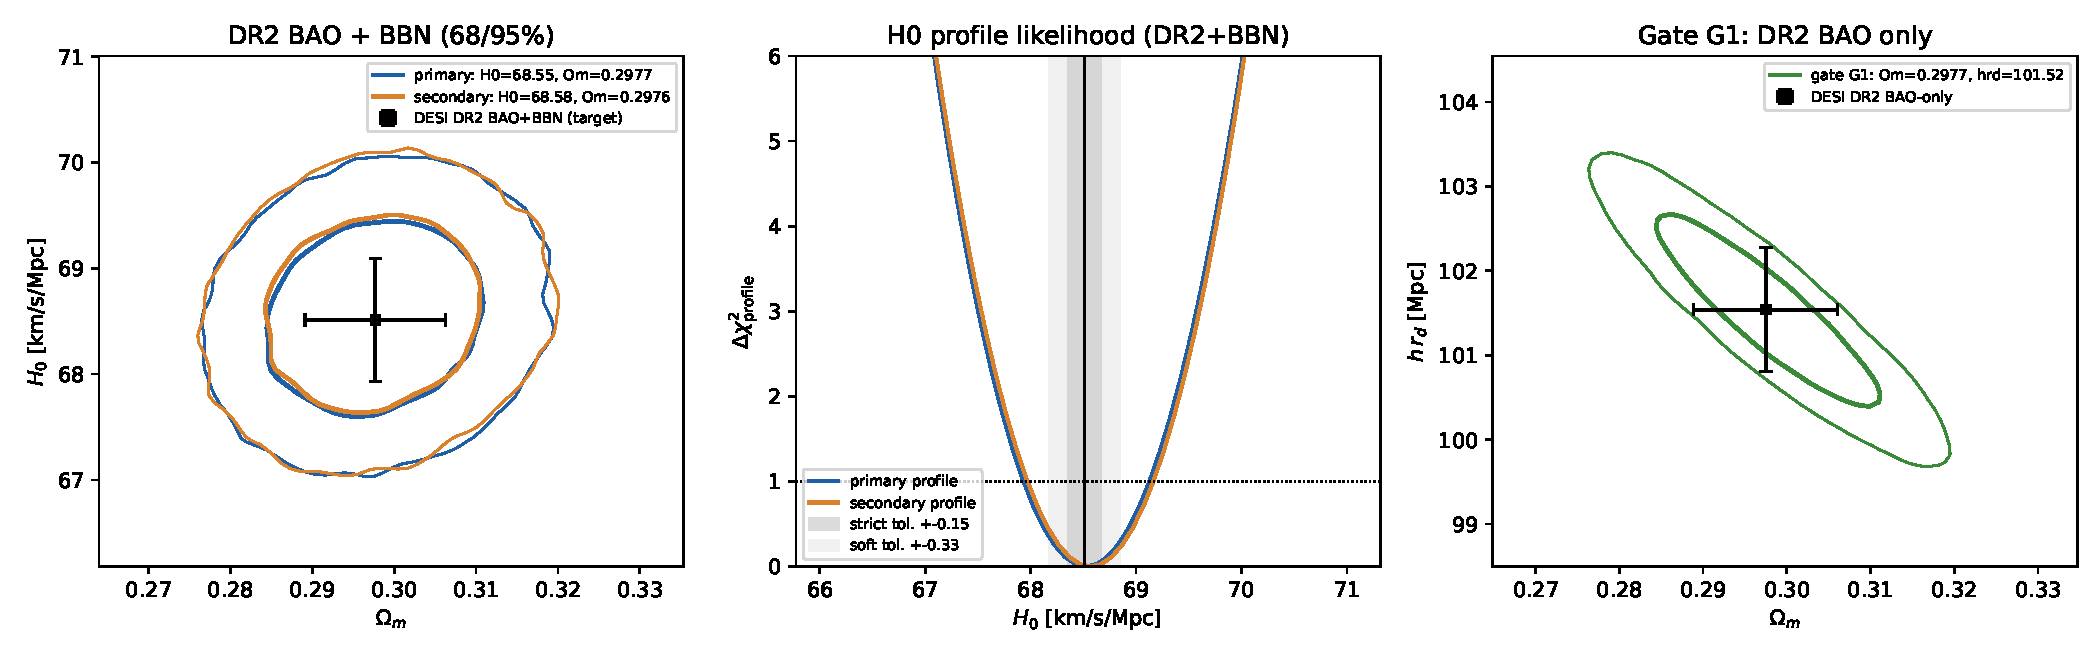
\includegraphics[width=\textwidth]{../../results/bao_bbn_h0/bao_bbn_h0_fit.pdf}
\caption{Left: DR2 BAO+BBN posterior (68/95\%) for both analyses, with the
DESI DR2 DESI+BBN target. Centre: $H_0$ profile likelihood, with the strict
and soft tolerance bands shaded. Right: the G1 BAO-only gate in
$(\Omega_m, h r_d)$ against DESI DR2 eq.~17.}
\label{fig:fit}
\end{figure}

\section{Lean 4 formalization}

\texttt{formal/ANSE/BAO\_BBN\_H0.lean} (sha256 \texttt{\LeanShaShort\ldots})
states exact facts about the \emph{model as coded} in
\texttt{scripts/bao\_bbn\_h0/common.py}. It uses pinned Mathlib imports
(\texttt{Analysis.Real.Sqrt}, \texttt{SpecialFunctions.Pow.Real},
\texttt{Convex.SpecificFunctions.Basic},
\texttt{Tactic.\{Positivity,Linarith,Ring\}}) and no \texttt{import Mathlib}.
The definitions, verbatim:
\begin{lstlisting}[mathescape]
noncomputable def omegaNu : $\mathbb{R}$ := 0.0107 * 0.06

noncomputable def rdAubourg (wcb wb : $\mathbb{R}$) : $\mathbb{R}$ :=
  55.154 * Real.exp (-72.3 * (omegaNu + 0.0006) ^ 2) /
    (wcb ^ (0.25351 : $\mathbb{R}$) * wb ^ (0.12807 : $\mathbb{R}$))

noncomputable def omegaCb (h Om : $\mathbb{R}$) : $\mathbb{R}$ := Om * h ^ 2 - omegaNu

noncomputable def H0 (h : $\mathbb{R}$) : $\mathbb{R}$ := 100 * h

noncomputable def DH_over_rd (c h E rd : $\mathbb{R}$) : $\mathbb{R}$ := c / H0 h / E / rd
\end{lstlisting}

The \LeanNThm{} theorem statements, verbatim (proofs elided):
\begin{lstlisting}[mathescape]
theorem rd_numerator_pos : 0 < 55.154 * Real.exp (-72.3 * (omegaNu + 0.0006) ^ 2) := ...

theorem rdAubourg_pos {wcb wb : $\mathbb{R}$} (hcb : 0 < wcb) (hb : 0 < wb) :
    0 < rdAubourg wcb wb := ...

theorem rdAubourg_strictAntiOn_cb {wb : $\mathbb{R}$} (hb : 0 < wb) :
    StrictAntiOn (fun wcb => rdAubourg wcb wb) (Set.Ioi (0 : $\mathbb{R}$)) := ...

theorem rdAubourg_strictAntiOn_b {wcb : $\mathbb{R}$} (hcb : 0 < wcb) :
    StrictAntiOn (rdAubourg wcb) (Set.Ioi (0 : $\mathbb{R}$)) := ...

theorem rd_strictAntiOn_Om {h wb : $\mathbb{R}$} (hh : 0 < h) (hb : 0 < wb) :
    StrictAntiOn (fun Om => rdAubourg (omegaCb h Om) wb) {Om : $\mathbb{R}$ | 0 < omegaCb h Om} := ...

theorem DH_over_rd_eq_hrd (c h E rd : $\mathbb{R}$) :
    DH_over_rd c h E rd = c / (100 * (h * rd) * E) := ...

theorem DH_over_rd_degenerate {h rd h' rd' : $\mathbb{R}$} (c E : $\mathbb{R}$) (hprod : h * rd = h' * rd') :
    DH_over_rd c h E rd = DH_over_rd c h' E rd' := ...

theorem gate_reparam_exact {hrad : $\mathbb{R}$} (hne : hrad $\neq$ 0) (c E hrd : $\mathbb{R}$) :
    DH_over_rd c hrad E (hrd / hrad) = c / (100 * hrd * E) := ...

theorem hrd_mono_generic {a w Om h1 h2 : $\mathbb{R}$} (ha : 0 < a) (ha3 : a $\le$ 1 / 3) (hw : 0 < w)
    (hOm : 0 < Om) (hh1 : 0 < h1) (h12 : h1 < h2) (hsupp : w $\le$ (1 - 2 * a) * (Om * h1 ^ 2)) :
    h1 * (Om * h2 ^ 2 - w) ^ a < h2 * (Om * h1 ^ 2 - w) ^ a := ...

theorem hrd_strictMonoOn_h {Om wb : $\mathbb{R}$} (hOm : 0 < Om) (hb : 0 < wb) :
    StrictMonoOn (fun h => h * rdAubourg (omegaCb h Om) wb)
      {h : $\mathbb{R}$ | 0 < h $\wedge$ omegaNu $\le$ (1 - 2 * 0.25351) * (Om * h ^ 2)} := ...
\end{lstlisting}

In words, the theorems say the following.
\begin{itemize}
\item Eq.~\eqref{eq:aub} is positive, and strictly decreasing in
  $\omega_{cb}$ and in $\omega_b$, on $(0,\infty)$.
\item At fixed $h$ and $\omega_b$, $r_d$ is strictly decreasing in
  $\Omega_m$ on the sampled support $\{\Omega_m h^2-\omega_\nu>0\}$.
\item At fixed $E$, the coded $D_H/r_d$ equals $c/[100(h r_d)E]$.
\item The gate's substitution $r_d\mapsto h r_d/h_\mathrm{rad}$ at fixed
  $h_\mathrm{rad}\neq0$ is an exact reparametrisation.
\item Identifiability (secondary $r_d$): at fixed $\Omega_m>0$ and
  $\omega_b>0$, $h\mapsto h\,r_d(\Omega_m h^2-\omega_\nu,\omega_b)$ is
  strictly increasing on $\{h>0:\omega_\nu\le(1-2a)\Omega_m h^2\}$ with
  $a=0.25351$. Once BAO fix $(\Omega_m, h r_d)$ and BBN fixes $\omega_b$, at
  most one $h$ on that set matches. The proof uses Bernoulli's inequality with exponent
  $a/(1-2a)\le1$.
\end{itemize}
The identifiability hypothesis is stronger than the preregistered bare
``$1-2a>0$'', because $\omega_\nu>0$ is subtracted inside the power. It is
needed: for eq.~\eqref{eq:aub}, $h\,r_d$ is \MonoBelowDec{} in $h$ below
$\omega_m=\MonoThr$. It holds wherever $\Omega_m h^2\ge\MonoThr$, which
includes the T1 posterior by a wide margin ($\omega_m\approx0.14$). It does
not hold on the whole secondary prior support: the band
$\omega_\nu<\Omega_m h^2<\MonoThr$ (e.g.\ $\Omega_m\approx0.01$ with $H_0$
of 25--36) is sampled, and there $h\,r_d$ decreases. The CAMB table's
$\omega_{cdm}\ge0.005$ support excludes that corner for the primary. As a numerical
companion, $h\,r_d(h)$ is strictly increasing on \MonoAllOk{} \MonoN{}
sampled curves per box, in the T1 $\pm5\sigma$ box and in a wide box, for
both the eq.~16 and the CAMB-table $r_d$
(\texttt{fixround\_diagnostics.json}). The Lean theorem covers eq.~16 only.

The \texttt{\#print axioms} lines are part of the source file, so the check
is reproducible from the source (the Elenchus \texttt{NO\_FOOTPRINT} rule).
The fix round re-ran the compile read-only against the main checkout's
build. Its first attempt failed with five errors (logged). The second
attempt compiled. Its raw output:
\begin{verbatim}
# started_utc: 2026-09-27T19:01:59Z
# source_sha256: 2b6530838efa0df9bfb475a5d8b25ee29aa121989cc83d04e07f595f5f616e38
'ANSE.BAOBBNH0.rd_numerator_pos'
    depends on axioms: [propext, Classical.choice, Quot.sound]
'ANSE.BAOBBNH0.rdAubourg_pos'
    depends on axioms: [propext, Classical.choice, Quot.sound]
'ANSE.BAOBBNH0.rdAubourg_strictAntiOn_cb'
    depends on axioms: [propext, Classical.choice, Quot.sound]
'ANSE.BAOBBNH0.rdAubourg_strictAntiOn_b'
    depends on axioms: [propext, Classical.choice, Quot.sound]
'ANSE.BAOBBNH0.rd_strictAntiOn_Om'
    depends on axioms: [propext, Classical.choice, Quot.sound]
'ANSE.BAOBBNH0.DH_over_rd_eq_hrd'
    depends on axioms: [propext, Classical.choice, Quot.sound]
'ANSE.BAOBBNH0.DH_over_rd_degenerate'
    depends on axioms: [propext, Classical.choice, Quot.sound]
'ANSE.BAOBBNH0.gate_reparam_exact'
    depends on axioms: [propext, Classical.choice, Quot.sound]
'ANSE.BAOBBNH0.hrd_mono_generic'
    depends on axioms: [propext, Classical.choice, Quot.sound]
'ANSE.BAOBBNH0.hrd_strictMonoOn_h'
    depends on axioms: [propext, Classical.choice, Quot.sound]
rc=0
\end{verbatim}

There is no \texttt{sorryAx}, and every footprint is the trusted set.
\textsc{SocrateAI-Scientific-Elenchus} \texttt{elenchus\_check.py} reported
\texttt{no findings}. A copy with the identifiability proof replaced by
\texttt{sorry} also compiled with exit code~0 but showed \texttt{sorryAx}
in its footprint. So the axiom-set rule, not the exit code, is the gate.

\paragraph{Scope.}
The theorems say nothing about the CAMB $r_d$ of the primary analysis, and
nothing about any fitted number. $E$ enters as a free real. In the BBN fits,
$E(z)$ depends on $h$ through the radiation term. The ``only through
$h r_d$'' identity is therefore exact at fixed $E$: for the gate, where
$E$ is evaluated at fixed $h_\mathrm{rad}$. For the full BBN likelihood it
holds only up to that radiation dependence, of order $10^{-4}$. The Lean
docstrings and ledger glosses now say ``at fixed $E$''. The match between the Lean definitions and the Python code is a
reading, filed as a Tier~C claim below, not a kernel fact.

\paragraph{Content and deviation from the Lean plan.}
Six theorems are substantive. They are positivity of eq.~\eqref{eq:aub},
its strict monotonicity in $\omega_{cb}$, $\omega_b$ and $\Omega_m$, and
\texttt{hrd\_mono\_generic} with \texttt{hrd\_strictMonoOn\_h}, the
preregistered ``$h\,r_d(h)$ strictly increasing in $h$''. An earlier draft
lacked the last one. It was added in the fix round, with the strengthened
hypothesis described above. The other four theorems are
\texttt{rd\_numerator\_pos} (positivity of a numeric constant) and three
field identities in which $E$ is a free real (\texttt{DH\_over\_rd\_eq\_hrd},
\texttt{DH\_over\_rd\_degenerate}, \texttt{gate\_reparam\_exact}).

\section{Claim ledger}

All quantitative claims are registered in an Elenchus tier-capped ledger
(\texttt{results/bao\_bbn\_h0/ledger/}): \LedgerClaims{} claims, each with
a content-addressed evidence blob. The tiers:
\begin{itemize}
\item \textbf{A:} the \LeanNThm{} Lean theorems;
\item \textbf{B:} fits, controls and instrument checks;
\item \textbf{L:} published values, and every comparison with them,
  including the PASS/PARTIAL verdicts;
\item \textbf{C:} the Lean-to-code correspondence.
\end{itemize}
The gate (\texttt{ledger.py -{}-evidence-dir}) reports \LedgerBlock{}
block findings and \LedgerFlag{} \texttt{LEDGER\_UNAUDITED\_TIER\_A}
flags, with exit code \LedgerRc. The gate returns a non-zero code
whenever any finding exists, flags included, so the non-zero exit comes
only from those flags. The eight Tier~A rows that existed at review carry
an audit object from the fix-round \emph{model} referee, which judged
every statement faithful. The object's \texttt{by} field says so, and the
evidence is \texttt{ledger/referee\_statement\_audit\_fixround.json}.
Elenchus defines an audit as a person's certification, so these rows are
model-audited only. No person has audited any statement. The two
identifiability theorems were added after that review. Their rows keep
\texttt{audit: null}, and those are the open flags. An older model review,
\texttt{ledger/referee\_statement\_audit.json}, is not used.

Three hand-built mutations were each caught:
\begin{itemize}
\item the headline verdict refiled as Tier~B (tier inversion);
\item a one-byte change to an evidence blob (evidence mismatch);
\item a citation refiled as Tier~A (kind overclaim).
\end{itemize}

\section{Limitations}

\begin{itemize}
\item \textbf{A reproduction, not a new result.} We use DESI's data vector,
  BBN prior and flat priors, so agreement is expected if both pipelines are
  correct. It tests our pipeline, not cosmology.
\item \textbf{The DR1 second check is PARTIAL.} A propagation of the
  DR1-quoted $h r_d$ makes a DESI-side rounding difference plausible, but
  this was not tested.
\item \textbf{Model dependence.} The result assumes flat $\Lambda$CDM,
  $N_\mathrm{eff}=3.044$ and standard recombination. The
  $N_\mathrm{eff}=4.044$ demonstration shifts $H_0$ by \SensNeff.
\item \textbf{Instrument details.}
  \begin{itemize}
  \item The primary $r_d$ is interpolated from a CAMB table, not computed
    per likelihood call.
  \item \NSubst{} table nodes far from the posterior were refilled at a
    neighbouring $h$.
  \item The table's support truncates the flat $H_0$ prior at 99. This is
    relevant only for N3.
  \item G1 and G2 evaluate radiation at a fixed $h$.
  \end{itemize}
\item \textbf{Eq.~16 accuracy.} The measured deviation of eq.~16 from CAMB
  (\AubMaxAbs\%) exceeds its stated 0.021\% at $N_\mathrm{eff}=3.044$. Part
  of this is the uncorrected $N_\mathrm{eff}$ offset. The effect on $H_0$
  is the measured \DPrimSecOne.
\item \textbf{Repository checks} (re-run in the fix round; raw logs in
  \texttt{results/bao\_bbn\_h0/}).
  \begin{itemize}
  \item \texttt{test\_rigor\_guard.py}: all \RigorFiles{} files pass the
    anti-stub check.
  \item \texttt{antigravity\_guard.py}: \AgStatus, with \AgFlags{}
    ``hallucinated import'' flags repository-wide, \AgOwnFlags{} of them in
    \texttt{scripts/bao\_bbn\_h0/}. The failure comes from files outside
    this problem.
  \item \texttt{pytest tests/} (worktree \texttt{.venv}): \PyResult.
    No test covers \texttt{scripts/bao\_bbn\_h0/}, so these results say
    nothing about this analysis either way.
  \end{itemize}
\item \textbf{No human review.} No person has reviewed this paper or
  audited the Lean statements. Eight Tier~A rows carry a model referee's
  audit, and two carry none.
\end{itemize}

\section*{Reproducibility}
Scripts live in \texttt{scripts/bao\_bbn\_h0/}:
\begin{itemize}
\item \texttt{rd\_camb\_table.py}, \texttt{controls.py},
  \texttt{fit\_real.py} and \texttt{make\_figure.py} produce the fit;
\item \texttt{lean\_recheck.py}, \texttt{write\_lean\_verification.py},
  \texttt{build\_ledger.py} and \texttt{ledger\_gate\_check.py} produce the
  ledger;
\item \texttt{fixround\_diagnostics.py} and \texttt{control\_n4.py} produce
  the fix-round diagnostics and the post-hoc control N4;
\item \texttt{make\_paper\_inputs.py} generates every number in this paper.
\end{itemize}
The \texttt{fit.json} used here has sha256 prefix
\texttt{\FitShaShort}. MCMC chains are stored off-repository, and their
sha256 are listed in \texttt{results/bao\_bbn\_h0/chains\_pointer.json}.
Software: CAMB~\CambVer, classy~3.3.4, emcee, astropy, numpy and scipy.

\begin{thebibliography}{9}

\bibitem{desi2025dr2}
DESI Collaboration, arXiv:2503.14738 (2025); eqs.~(2), (14), (17), (19), Table~V.

\bibitem{desi2024vi}
DESI Collaboration, arXiv:2404.03002 (2024); eqs.~(2.8), (4.4), Tables~2--3, Sec.~8.

\bibitem{aubourg2015}
Aubourg et al., arXiv:1411.1074 (2015); eqs.~16--17.

\bibitem{schoeneberg2024}
N.~Sch\"oneberg, arXiv:2401.15054 (2024); eq.~(5.1).

\bibitem{schoeneberg2022}
N.~Sch\"oneberg et al., arXiv:2209.14330 (2022); Sec.~2.1.1.

\bibitem{planck2018}
Planck Collaboration, arXiv:1807.06209 (2018); Tables~1--2.

\end{thebibliography}

\end{document}
